\documentclass[a4paper]{article}

\usepackage[portuguese]{babel}
\usepackage[T1]{fontenc}
\usepackage[utf8]{inputenc}
\usepackage{hyperref}
\usepackage{graphicx}
\usepackage{float}
\usepackage[hypcap]{caption} % makes \ref point to top of figures and tables
\usepackage{amsmath}
\usepackage[nottoc,numbib]{tocbibind}	% adds Biliography to index
%\usepackage[margin=3.3cm]{geometry}

\begin{document}

\pagenumbering{gobble}	% disable page numbering
\begin{titlepage}

	\begin{center}

		
\includegraphics[width=6cm]{./title}\\[3cm]

		\textsc{\LARGE Segurança Informática em Redes e Sistemas}\\[1.5cm]

		\textsc{\Large Projecto}\\[1.5cm]


		{ \huge \bfseries Zero-Day Vulnerability \\[2.5cm] }


		\noindent
		\begin{center} \large
			Gonçalo Ribeiro, 73294\\[5mm]

			António Bacelar de Sousa, 73425\\[5mm]

			Rafael Gonçalves, 73786\\[2.5cm]

		\end{center}

		\begin{minipage}{0.4\textwidth}
			\begin{flushleft} \Large
				Prof. Ricardo Chaves
			\end{flushleft}
		\end{minipage}
		\begin{minipage}{0.4\textwidth}
			\begin{flushright} \Large
				Prof. Miguel Pardal
			\end{flushright}
		\end{minipage}

		\vfill

		{\large \today}

	\end{center}

\end{titlepage}

\tableofcontents
\pagebreak

\pagenumbering{arabic}
\section{Motivação}
Este trabalho tem como motivação fazer um estudo aprofundado de uma \textit{zero-day vulnerability}, e, desta forma, perceber como funcionam este tipo de ataques e como são tratadas as vulnerabilidades a eles associadas. Para além disso, como motivação também surge o facto de esta ser uma oportunidade para aplicar os conhecimentos adquiridos este semestre na disciplina de Segurança Informática em Redes e Sistemas.

\pagebreak
\section{Objectivos}
\label{sec:objectivos}

\subsection{Antes de 25 de Novembro}

\subsection*{Básico}
Especificar uma vulnerabilidade no Haihaisoft Universal Player.
\subsection*{Intermédio}
Realização de um ataque ao software por intermédio da vulnerabilidade especificada.
\subsection*{Avançado}
Investigação e aplicação de métodos que permitam resolver total ou parcialmente a vulnerabilidade do Haihaisoft UP.

\subsection{Após 25 de Novembro}
Após uma análise cuidada e tentativas de ataque ao Haihaisoft UP chegou-se à conclusão de que era inviável fazer uma \textit{exploit} que fosse consistente entre versões do Windows. Vimo-nos portanto obrigados a escolher outro software com uma vulnerabilidade \textit{zero-day}. De forma a aproveitar o conhecimento adquirido escolheu-se um software também vulnerável a \textit{buffer overflows}: o i.FTP. Seguem-se os novos objectivos.

\subsection*{Básico}
Especificar uma vulnerabilidade no software i.FTP.
\subsection*{Intermédio}
Realização de um ou vários ataques ao software tirando proveito da vulnerabilidade especificada.
\subsection*{Avançado}
Tentar eliminar a vulnerabilidade estudada.


\pagebreak
\section{Plano de Trabalho}

\subsection{Semana 1}
Prazo: 07/11/14
\subsubsection{Disponibilidade}
Reduzida devido a avaliações e entregas de projectos de outras UCs.

\subsubsection{Tarefas}
\begin{itemize}
\item escolher um software/website com uma vulnerabilidade activa
\item definir os parâmetros iniciais do projecto
\end{itemize}

\subsubsection{Trabalho Realizado}
Nesta semana procuram-se listas de software/websites com vulnerabilidades activas e foi escolhido o Haihaisoft Universal Player\footnote{\url{http://www.haihaisoft.com/hup.aspx}}, um leitor universal de ficheiros multimédia, como objecto de estudo deste projecto. Este software é desenvolvido para Windows e é software aberto.

Foram também delineados os objectivos deste projecto (Secção~\ref{sec:objectivos}).

\subsection{Semana 2}
Prazo: 14/11/14
\subsubsection{Disponibilidade}
Reduzida devido a avaliações e entregas de projectos de outras UCs.

\subsubsection{Tarefas}
\begin{itemize}
\item preparar uma máquina virtual que possa ser usada ao longo do projecto;
\item testar a \textit{proof of concept} (POC) da vulnerabilidade \textit{zero-day}.
\end{itemize}

\subsubsection{Trabalho Realizado}
Tendo-se verificado que o Haihaisoft Universal Player funciona exclusivamente em Windows, foi esse o sistema operativo escolhido para instalar na máquina virtual. Como o Windows é software pago teve-se em conta esse factor de forma a fazer uma instalação que não tivesse problemas com licenças. Neste sentido, e visto que o Windows 10 Technical Preview foi lançado recentemente, foi esta a versão do Windows que se escolheu instalar na máquina virtual. De seguida instalou-se o Haihaisoft UMP e verificou-se o seu correcto funcionamento.

Uma das coisas que impressionou foi o facto de o Haihaisoft UP precisar de privilégios de administrador para ser executado. Como tal, e visto que este software é vulnerável a buffer overflows, o código que se conseguiu injectar vai correr com privilégios de administrador deixando a máquina largamente à mercê de potenciais atacantes.

Por fim testou-se a POC encontrada na Exploit Database\footnote{\url{http://www.exploit-db.com/exploits/32514/}}. Esta POC consiste num pequeno \textit{script} escrito em Python. Como tal, instalou-se Python na máquina virtual. Tentámos correr o \textit{script}, mas o código Python revelava alguns erros. Após correcção desses erros conseguiu-se gerar 3 ficheiros de \textit{exploit}. Experimentou-se então abrir esses ficheiros no Haihaisoft UP. Os resultados dos 3 ficheiros foram semelhantes: com um deles o programa fechou-se mal era aberto; com os outros dois ficheiros o programa deixava de responder (aparecia o menu do Windows a dar essa informação), e passado algum tempo o programa era fechado. O \textit{shellcode} introduzido é um conjunto de instruções que ainda não houve oportunidade de verificar o que faz. No entanto verificou-se que claramente algo de errado acontece com o programa ao abrir os ficheiros de \textit{exploit}.

\subsection{Semana 3}
Prazo: 21/11/14
\subsubsection{Disponibilidade}
Muito reduzida devido ao teste de SIRS.

\subsubsection{Tarefas}
\begin{itemize}
	\item Identificar o objectivo do código Assembly injectado através de \textit{buffer overflow}.
\end{itemize}

\subsubsection{Trabalho Realizado}
%Examinou-se o código fonte de maneira a descobrir o endereço de retorno, de maneira a alterar o código de exploit para correr código feito pelo grupo

Nesta semana foi analisada a POC. São escritos bytes com 4 valores diferentes para o ficheiro de \textit{exploit}. Chegou-se à conclusão de que os valores dos bytes se referem aos caracteres ASCII A, B e C e que o outro valor é usado como \textit{padding}.

\subsection{Semana 4}
Prazo: 28/11/14
\subsubsection{Disponibilidade}
Maior disponibilidade.
\subsubsection{Tarefas}
\begin{itemize}
	\item Desenvolvimento do código que se serve da vulnerabilidade encontrada para conseguir acesso com privilégios elevados.
\end{itemize}

\subsubsection{Trabalho Realizado}
A primeira conclusão a que se chegou foi que não é possível fazer um \textit{stack based overflow}. O Windows usa SEH (\textit{structured exception handlers}) o que faz com que \textit{stack based overflows} não sejam possíveis, ou seja, fazer um overwrite directo do EIP (instruction pointer) e fazer um RET.

Outra conclusão a que se chegou foi que o \textit{buffer} cuja capacidade é excedida não é directamente o \textit{buffer} que recebe a URL, mas sim um \textit{buffer} que contém a URL transformada, após transformação/eliminação de caracteres que não são permitidos em URLs. Isto significa que os valores de bytes que são possíveis escrever ficam muito mais limitados. Mais concretamente de 256 valores de bytes passa-se a poder usar apenas cerca de 90 valores. Por outro lado não é possível usar o valor \texttt{0x00} porque é o terminador de \textit{strings}, e portanto ao usar o programa este pára de copiar bytes assim que encontra um byte com esse valor (parando o overflow antes do que se quer).

O Haihaisoft UP não foi compilado com protecção da SEH. Ou seja em teoria é possível fazer \textit{overflow} das estruturas SEH e enganar o programa de forma a que escreva um novo valor no EIP, valor esse escolhido pelo grupo. Para fazer isto tem que se conseguir que o programa execute uma sequência de instruções POP POP RET, que tem que estar em código não compilado com protecção de SEH. Neste caso, o próprio executável não tem esta protecção pelo que esta sequência de instruções podia ser uma do próprio programa.

Os programas em Windows têm a memória dividida em 3 componentes. Entre estas, a componente de código é aquela que tem as instruções do programa. Ou seja, é lá que se tem que encontrar uma sequência POP POP RET. No entanto, verificou-se que os endereços de memória do segmento de código começam todos pelo byte \texttt{0x00}. Isto significa que para enganar o programa de forma a que este salte para a dita sequência de código, teria-se que fazer um overwrite da SEH handler para um endereço cujo primeiro byte é \texttt{0x00}. Ora isso não é possível porque não é possível escrever esse valor de byte. Portanto, não se consegue que seja executada a sequência de instruções necessária para que se conseguísse alterar o EIP para uma zona de memória controlada pelo grupo de forma a executar uma \textit{exploit}.

Decidiu-se então alterar o alvo de estudo do nosso projecto do Haihaisoft UMP para outro zero-day.


\subsubsection{Novo Paradigma -- i.FTP}
Consultou-se a Exploit Database\footnote{\url{http://www.exploit-db.com}} de forma a encontramos um \textit{zero-day} novo. O candidato escolhido foi o i.FTP\footnote{\url{http://www.memecode.com/iftp.php}}. Trata-se de um cliente de FTP que apresenta vulnerabilidades de \textit{buffer overflow} (foi decidido manter o tipo de vulnerabilidade a ser explorada).

O referido site oferece uma POC para esta vulnerabilidade. Após análise dessa POC conclui-se que a vulnerabilidade resulta do carregamento de um ficheiro de configurações do programa -- Schedule.xml \footnote{localizado em C:\textbackslash Users\textbackslash someuser\textbackslash AppData\textbackslash Local\textbackslash VirtualStore\textbackslash Program Files (x86)\\ \textbackslash Memecode\textbackslash i.Ftp}. Existe um campo nesse ficheiro que se refere ao tempo para o qual se quer agendar uma transferência. Esse campo é susceptível a \textit{overflows}.

Foi feita uma análise da vulnerabilidade e conseguimos executar uma \textit{exploit} (abrir a calculadora do Windows). Esta \textit{exploit} não é muito interessante e portanto vai-se tentar elaborar outra que o seja.

Ao correr o programa a calculadora é imediatamente aberta e o programa termina com a janela do Windows que diz que o programa não responde. Gostava-se que fosse possível evitar que o programa terminasse de forma a que não seja perceptível que algo de errado se passou. A calculadora não é afectada pela terminação do i.FTP, ou seja a \textit{exploit} continua a correr mesmo com o fecho do i.FTP.


\subsection{Semana 5}
Prazo: 05/12/14
\subsubsection{Disponibilidade}
Média.
\subsubsection{Tarefas}
\begin{itemize}
	\item Elaborar um ataque mais interessante;
	\item Evitar que o programa deixe de responder;
	\item Tentar eliminar a vulnerabilidade;
	\item Conclusão do presente documento.
\end{itemize}


\section{SEH Based Overflow -- Passo a Passo}

Nem sempre é possível fazer uma \textit{stack based exploit}. No entanto no Windows às vezes é possível fazer um ataque com base na SEH (\textit{structured exception handling}). A SEH é basicamente uma lista ligada de registos relativos às excepções de um programa. Mesmo que um programa não tenha \textit{exception handling} existe sempre uma handle na SEH que pertence ao Windows e é usada se a excepção não for apanhada por outra handle da SEH.

Cada registo da SEH tem dois ponteiros: um deles aponta para o código a correr no caso da excepção se verificar (SE handler); o outro aponta para a estrutura seguinte da SEH.

A função que é chamada no caso de ocorrer uma excepção tem a particularidade de receber quatro argumentos, sendo que um desses argumentos é a ``\textit{establisher frame}'' cujo valor é o endereço em que se encontra o endereço para a próxima estrutura da SEH. Este endereço é o terceiro elemento no topo da pilha quando a função é chamada. Isto significa que se após a chamada da função for executada uma sequência de instruções POP POP RET, o registo EIP passa a apontar para o endereço imediatamente antes da SE handler. Há portanto a possibilidade de se conseguir executar código visto que com o \textit{overflow} é possível controlar tanto o valor da SE handler como o valor do ponteiro para a próxima estrutura da SEH.

Os passos necessários para fazer uma SEH \textit{based exploit} são:

\begin{enumerate}
	\item descobrir aproximadamente a partir de que tamanho de input o programa termina inesperadamente -- exemplo: o programa não apresenta problemas com um input de 1000 caracteres mas sim com um de 2000;
	\item verificar se o programa é vulnerável a ataques via SEH -- se não for não vale a pena continuar;
	\item determinar o textit{offset} da SEH;
	\item encontrar um endereço com uma sequência de instruções POP POP RET;
	\item verificar qual a melhor localização da stack para escrever o \textit{shellcode};
	\item escrever as instruções necessária para fazer um ou vários saltos até à localização do \textit{shellcode};
	\item escrever o \textit{shellcode}, sem caracteres terminadores e outros que não seja possível usar;
	\item testar a \textit{exploit}.
\end{enumerate}

De seguida descreve-se brevemente como se pode executar cada passo. O debugger usado é o Immunity Debugger. Outro programa auxiliar é o Metasploit.

\paragraph*{Programa vulnerável a SEH?} Usando o plugin \texttt{mona} é possível determinar facilmente quais os módulos não compilados com SafeSEH. Para tal, após instalação do \texttt{mona} basta executar o seguinte comando:

	\texttt{!mona nosafeseh}

No caso do i.FTP é perceptível que existem dois módulos carregados pelo programa que não têm SafeSEH: \texttt{iftp.exe} e \texttt{Lgi.dll}. Pode-se também ver quais os endereços de memória do seu código.

\paragraph*{Determinar \textit{offset} da SEH} O \textit{offset} da SEH pode ser determinado com o auxílio do comando \texttt{pattern-create} da ferramenta do Metasploit. Esta ferramenta gera uma sequência de bytes sem repetições, em que se torna fácil descobrir o offset de conjuntos de vários bytes.

	\texttt{ruby pattern\_create.rb 2000}

2000 deve ser substituído pelo número de bytes que se quiser para a sequência. Esse valor deve ser suficientemente grande para que o programa termine inesperadamente.

Usando o debugger para examinar o \textit{overflow} podemos verificar qual o valor escrito no ``Pointer to the next SEH record'' (nSEH). O \textit{offset} desse valor desde o início do \textit{buffer} pode depois ser obtido com:

	\texttt{ruby pattern\_offset.rb Au0A}

em que Au0A é o valor escrito no sítio do ponteiro anteriormente referido para no caso do i.FTP. Ficou-se a saber que o offset do início da estrutura é 600.

\paragraph*{Encontrar POP POP RET} Tem que se encontrar uma sequência POP POP RET num dos módulos que não tenha SafeSEH. Existem várias formas de o fazer. A mais simples é pesquisar uma sequência de comandos no disassembler fazendo \textit{Search for > Sequence of commands (CTRL + S)} e escrever nessa janela o que se pode ser na Figura~\ref{find_POPPOPRET}.

\begin{figure}
	\centering
	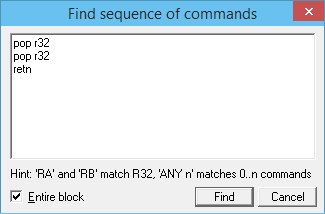
\includegraphics[scale=1]{find_POPPOPRET}
	\caption{procurar uma sequência POP POP RET}
	\label{find_POPPOPRET}
\end{figure}

Uma vez encontrada essa sequência há que anotar o seu endereço para o usar mais tarde. Neste caso anotou-se \texttt{0x1001A24A}, pertencente ao \texttt{Lgi.dll}.

\paragraph*{Melhor localização para o \textit{shellcode}} A melhor localização para o código do shellcode varia com a sua dimensão e qual o número de bytes na \textit{stack} que se tem sob controlo. No caso do i.FTP o \textit{offset} do último byte sobre o qual se tem controlo é cerca de 1360 pelo que devemos ter espaço que chegue para o \textit{shellcode} a seguir ao registo da SEH. Deferimos então que o \textit{shellcode} será colocado a seguir ao registo da SEH que está sob nosso controlo.

\paragraph*{Escrever instrução de salto} Para este passo existem várias opções. É possível fazer compilar uma instrução de salto e usá-la. Mas como neste caso se trata apenas de uma instrução optou-se por usar uma referência de x86 para identificar o \textit{opcode} a usar. Só é necessário saltar para o endereço a seguir ao do registo da SEH. Para isso basta um salto de no máximo 8 bytes visto que esse é o tamanho total do registo da SEH. Foram consultados \cite{AMD64vol3_2013} e \cite{refx86asm} e chegou-se à conclusão de que para fazer um near JUMP o \textit{opcode} é \texttt{0xEB} e que o byte seguinte é o valor do salto.

No nSEH escreveu-se por exemplo \texttt{0xEB069090} ou \texttt{0x9090EB04} (\texttt{0x90} são NOPs), ou seja pode-se saltar ou 6 ou 4 bytes dependendo do alinhamento que se der à instrução near JUMP. A seguir à SEH começamos a escrever o \textit{shellcode} e é para lá que se vai saltar.

\paragraph*{Escrever o \textit{shellcode}} Para escrever a \textit{exploit} pode-se usar uma ferramenta do Metasploit, o \texttt{msfpayload}. Este programa gera vários \textit{shellcodes} para diferentes sistemas operativos.

Um exemplo clássico é o de um \textit{shellcode} que abre uma calculadora do Windows:

	\texttt{ruby msfpayload windows/exec CMD=calc.exe R}

No entanto, o \textit{shellcode} gerado pode conter alguns caracteres que não são é possíveis usar (caracteres terminadores de strings) e outros dependendo do caso. Os caracteres terminadores de strings são \texttt{0x00}, \texttt{0x0A} e \texttt{0x0D}. Tem que ser encontrado um \textit{shellcode} alternativo sem esses caracteres, o que pode ser feito com:

	\texttt{ruby msfpayload windows/exec CMD=calc.exe R | ruby msfencode \\ -b `\textbackslash x00\textbackslash x0A\textbackslash x0D' -t c}

Verificou-se que no caso do i.FTP outro caracter que parece terminar o overflow é o \texttt{0x26}, pelo que esse caracter também foi excluído.

O output resultante está pronto a ser usado como \textit{shellcode} para o SEH \textit{based overflow}.


\pagebreak
\section{Resultados}

\subsection{Esperados}
\subsection{Obtidos}


\pagebreak
\bibliographystyle{plain}
\nocite{CorelanTeam, refx86asm, genSEHexploits, AMD64vol3_2013}
\bibliography{CorelanTeam,refx86asm,genSEHexploits,AMD64vol3_2013}	% no spaces between commas!

\end{document}

